% !TEX root=./adl.tex

% -----------------------------------------------------------------------
\section{Mixture of Experts}

% =======================================================================
\subsection{Motivation and Basic Idea}

% -----------------------------------------------------------------------
\begin{frame}{MoE: High-Level Idea}

  \begin{center}
    \begin{tikzpicture}[
      scale=0.85, every node/.style={scale=0.85},
      box/.style={draw, rounded corners, fill=blue!8, minimum width=2.2cm, minimum height=0.55cm, align=center, font=\small},
      expert/.style={draw, rounded corners, fill=orange!15, minimum width=1.4cm, minimum height=0.5cm, align=center, font=\small},
      gate/.style={draw, rounded corners, fill=green!15, minimum width=1.6cm, minimum height=0.5cm, align=center, font=\small},
      arr/.style={-Stealth, thick},
    ]
      % Input
      \node[box] (input) at (0, 0) {Token $x$};

      % Router
      \node[gate] (router) at (0, 1.3) {Router $G(x)$};
      \draw[arr] (input) -- (router);

      % Experts
      \node[expert] (e1) at (-4, 3.0) {Expert 1};
      \node[expert] (e2) at (-2, 3.0) {Expert 2};
      \node[font=\large] at (0, 3.0) {$\cdots$};
      \node[expert] (en1) at (2, 3.0) {Expert $E{-}1$};
      \node[expert] (en) at (4, 3.0) {Expert $E$};

      % Router to experts (highlight active ones)
      \draw[arr, gray!40, thin] (router) -- (e1);
      \draw[arr, red!70!black, very thick] (router) -- (e2) node[midway, left, font=\scriptsize, red!70!black] {$g_2$};
      \draw[arr, gray!40, thin] (router) -- (en1);
      \draw[arr, red!70!black, very thick] (router) -- (en) node[midway, right, font=\scriptsize, red!70!black] {$g_E$};

      % Output combination
      \node[box] (output) at (0, 4.5) {$y = \sum_{i \in \text{top-}k} g_i(x) \cdot E_i(x)$};
      \draw[arr, gray!40, thin] (e1) -- (output);
      \draw[arr, red!70!black, very thick] (e2) -- (output);
      \draw[arr, gray!40, thin] (en1) -- (output);
      \draw[arr, red!70!black, very thick] (en) -- (output);

      % Annotation
      \node[font=\scriptsize, text=red!70!black, anchor=west] at (4.8, 1.3) {selects top-$k$ experts};
      \node[font=\scriptsize, text=gray, anchor=west] at (4.8, 3.0) {inactive experts (gray)};
    \end{tikzpicture}
  \end{center}

  \begin{itemize}
    \item Replace the dense FFN in each Transformer block with a \textbf{sparse MoE layer}
    \item Maintain $E$ expert sub-networks, each a standard FFN
    \item A \textbf{router} (gating network) selects the top-$k$ experts per token
    \item Output: weighted combination $y = \sum_{i \in \text{top-}k} g_i(x) \cdot E_i(x)$
  \end{itemize}
\end{frame}

% -----------------------------------------------------------------------
\begin{frame}{Why Mixture of Experts?}

  \begin{columns}
    \begin{column}{0.48\textwidth}
      \textbf{Dense models}: every parameter is used for every input token.
      \begin{itemize}
        \item Scaling parameters $\Rightarrow$ scaling FLOPs proportionally
        \item Training cost grows with model size
        \item Inference cost grows with model size
      \end{itemize}

      \vspace{0.5em}
      \textbf{Key insight}: Not all tokens need the same computation. Can we \emph{decouple} parameter count from compute cost?

      \vspace{0.5em}
      \textbf{Analogy}: Like consulting a team of specialists: you don't ask every expert for every question, only the relevant ones.
    \end{column}
    \begin{column}{0.48\textwidth}
      \begin{alertblock}{Mixture of Experts (MoE)}
        \begin{itemize}
          \item Maintain \emph{many} expert sub-networks
          \item For each token, activate only a \emph{few} experts
          \item $\Rightarrow$ Large model capacity with sparse computation
        \end{itemize}
      \end{alertblock}

      \vspace{0.3em}
      \textbf{Result}: Models with $N$ total parameters but only $\sim k/E \cdot N$ active parameters per token ($k$ active out of $E$ experts).

      \vspace{0.3em}
      \textbf{In practice}:
      \begin{itemize}
        \item Experts tend to \emph{specialize} on different token types, languages, or domains
        \item MoE models match dense model quality at $2$--$4\times$ less training compute
        \item Inference latency similar to a small dense model (only $k$ experts run)
        \item Most successful modern LLMs use MoE: Mixtral, DeepSeek-V3, Grok
      \end{itemize}
    \end{column}
  \end{columns}
\end{frame}

% -----------------------------------------------------------------------
\begin{frame}{Challenges of MoE}

  \begin{columns}
    \begin{column}{0.48\textwidth}
      \textbf{1.\ Top-$k$ is not differentiable}
      \begin{itemize}
        \item The discrete selection of which $k$ experts to activate is a hard, non-differentiable choice
        \item Gradients cannot flow through $\arg\!\mathrm{topk}$
        \item \textbf{Workaround}: Multiply each expert's output by its continuous gating weight $g_i(x)$. Gradients flow through $g_i$ via softmax over the selected experts
        \item Router weights $W_g$ are trained by the gating weights, not the selection decision
      \end{itemize}

      \vspace{0.3em}
      \textbf{2.\ Load balancing}
      \begin{itemize}
        \item Router tends to collapse: sends most tokens to a few ``favorite'' experts
        \item Favored experts improve faster $\Rightarrow$ attract even more tokens (self-reinforcing)
        \item Requires auxiliary losses or other mechanisms
      \end{itemize}
    \end{column}
    \begin{column}{0.48\textwidth}
      \textbf{3.\ Communication overhead}
      \begin{itemize}
        \item Experts distributed across GPUs
        \item Tokens must be dispatched to the right device via \textbf{all-to-all} communication
        \item Poor load balance $\Rightarrow$ stragglers and wasted compute
      \end{itemize}

      \vspace{0.3em}
      \textbf{4.\ Memory vs.\ compute trade-off}
      \begin{itemize}
        \item All expert weights must reside in memory, even though most are idle per token
        \item Total parameter count $\gg$ active parameters
        \item Inference requires careful memory management (e.g.\ expert offloading)
      \end{itemize}

      \vspace{0.3em}
      \textbf{5.\ Training instability}
      \begin{itemize}
        \item Router learning is noisy early in training
        \item Requires careful initialization and precision (e.g.\ router in \texttt{float32})
      \end{itemize}
    \end{column}
  \end{columns}
\end{frame}

% =======================================================================
\subsection{Sparsely-Gated MoE (Shazeer et al., 2017)}

% -----------------------------------------------------------------------
\begin{frame}{Sparsely-Gated MoE: Architecture}

  \cite{shazeer2017moe}: up to \textbf{131,072 experts}, top-$k$ gating ($k{=}2$).

  \begin{columns}
    \begin{column}{0.55\textwidth}
      \begin{center}
        \begin{tikzpicture}[
          scale=0.72, every node/.style={scale=0.72},
          box/.style={draw, rounded corners, fill=blue!8, minimum width=2.0cm, minimum height=0.55cm, align=center, font=\small},
          expert/.style={draw, rounded corners, fill=orange!15, minimum width=0.9cm, minimum height=0.5cm, align=center, font=\small},
          gate/.style={draw, rounded corners, fill=green!15, minimum width=2.6cm, minimum height=0.5cm, align=center, font=\small},
          arr/.style={-Stealth, thick},
        ]
          % Input
          \node[box] (input) at (0, 0) {Input $x$};

          % Noisy top-k router
          \node[gate] (router) at (0, 1.5) {Noisy gating $H(x){=}xW_g{+}\epsilon$\\ $G(x){=}\mathrm{softmax}(\mathrm{TopK})$};
          \draw[arr] (input) -- (router);

          % Experts
          \node[expert, fill=gray!15] (e1) at (-2.6, 3.3) {$E_1$};
          \node[expert] (e2) at (-1.3, 3.3) {$E_2$};
          \node[font=\large] at (0, 3.3) {$\cdots$};
          \node[expert, fill=gray!15] (en1) at (1.3, 3.3) {$E_{E{-}1}$};
          \node[expert] (en) at (2.6, 3.3) {$E_E$};

          % Router to experts (highlight active ones)
          \draw[arr, gray!40, thin] (router) -- (e1);
          \draw[arr, red!70!black, very thick] (router) -- (e2) node[midway, left, font=\scriptsize, red!70!black] {$G(x)_2$};
          \draw[arr, gray!40, thin] (router) -- (en1);
          \draw[arr, red!70!black, very thick] (router) -- (en) node[midway, right, font=\scriptsize, red!70!black] {$G(x)_E$};

          % Output combination
          \node[box] (output) at (0, 5.0) {$y = \sum_{i=1}^{E} G(x)_i\, E_i(x)$};
          \draw[arr, gray!40, thin] (e1) -- (output);
          \draw[arr, red!70!black, very thick] (e2) -- (output);
          \draw[arr, gray!40, thin] (en1) -- (output);
          \draw[arr, red!70!black, very thick] (en) -- (output);

          % Annotations
          \node[font=\scriptsize, text=red!70!black, anchor=west] at (3.2, 1.5) {selects top-$k$ experts};
          \node[font=\scriptsize, text=gray, anchor=west] at (3.2, 3.3) {inactive experts (gray)};
        \end{tikzpicture}
      \end{center}
    \end{column}
    \begin{column}{0.42\textwidth}
      \textbf{Placement in the LM} (5 layers):

      \vspace{0.3em}
      \begin{center}
        \begin{tikzpicture}[
          scale=0.7, every node/.style={scale=0.7},
          layer/.style={draw, rounded corners, fill=gray!12, minimum width=2.3cm, minimum height=0.45cm, align=center, font=\small},
          lstm/.style={draw, rounded corners, fill=blue!12, minimum width=2.3cm, minimum height=0.45cm, align=center, font=\small},
          moe/.style={draw, rounded corners, fill=orange!18, minimum width=2.3cm, minimum height=0.45cm, align=center, font=\small},
          arr/.style={-Stealth, thick},
        ]
          \node[layer] (emb) at (0, 0)   {Embedding (512)};
          \node[lstm]  (l1)  at (0, 0.9) {LSTM (512)};
          \node[moe]   (m)   at (0, 1.8) {MoE layer};
          \node[lstm]  (l2)  at (0, 2.7) {LSTM (512)};
          \node[layer] (sm)  at (0, 3.6) {Softmax};
          \draw[arr] (0, -0.7) -- (emb) node[midway, right, font=\scriptsize, gray] {word};
          \draw[arr] (emb) -- (l1);
          \draw[arr] (l1) -- (m);
          \draw[arr] (m) -- (l2);
          \draw[arr] (l2) -- (sm);
          \draw[arr] (sm) -- ++(0, 0.7);
        \end{tikzpicture}
      \end{center}

      \vspace{0.2em}
      \begin{itemize}
        \item A \emph{single} MoE layer between two LSTM layers
        \item Embedding, LSTM units, MoE input/output all dim \textbf{512}
        \item Each expert: FFN $512 \to 1024 \to 512$ (ReLU), $\approx$\,\textbf{1M params}
      \end{itemize}
    \end{column}
  \end{columns}
\end{frame}

% -----------------------------------------------------------------------
\begin{frame}{The Sparsely-Gated Mixture-of-Experts Layer}

  \textbf{Gating network} for input $x$:
  \[
    G(x) = \mathrm{softmax}\!\Big(\mathrm{TopK}\big(H(x),\, k\big)\Big)
  \]
  \[
    \mathrm{TopK}(v, k)_i =
    \begin{cases}
      v_i & \text{if } v_i \text{ is in the top } k \\
      -\infty & \text{otherwise}
    \end{cases}
  \]

  \textbf{Noisy gating} (training only, disabled at inference):
  \[
    H(x)_i = (x \cdot W_g)_i + \underbrace{\mathcal{N}(0,1) \cdot \mathrm{Softplus}\!\big((x \cdot W_{\text{noise}})_i\big)}_{\text{learned, input-dependent noise}}
  \]
  \begin{itemize}
    \item $W_{\text{noise}}$ is a second learned weight matrix controlling per-expert noise magnitude
    \item Noise encourages \emph{exploration}: prevents the router from always picking the same experts
    \item At inference, noise is turned off $\Rightarrow$ deterministic routing
  \end{itemize}

  \vspace{0.3em}
  \textbf{MoE output}: $y = \sum_{i=1}^{E} G(x)_i \cdot E_i(x)$ \quad (only $k$ terms non-zero)
\end{frame}

% -----------------------------------------------------------------------
\begin{frame}{Load Balancing}

  As discussed earlier, the router tends to collapse without intervention. Noisy gating helps but is not sufficient alone.

  \begin{columns}
    \begin{column}{0.55\textwidth}
      \textbf{Auxiliary load-balancing loss} (added to main loss):

      \vspace{0.2em}
      For a batch of $T$ tokens across $E$ experts:
      \begin{itemize}
        \item $f_i = \frac{1}{T} \sum_{t=1}^{T} \mathbbm{1}[\text{token } t \to \text{expert } i]$ \\ (hard, non-differentiable)
        \item $p_i = \frac{1}{T} \sum_{t=1}^{T} \mathrm{softmax}(H(x_t))_i$ \\ (soft, differentiable)
      \end{itemize}

      \[
        \mathcal{L}_{\text{bal}} = \alpha \cdot E \cdot \sum_{i=1}^{E} f_i \cdot p_i
      \]
      \[
        \mathcal{L} = \mathcal{L}_{\text{LM}} + \mathcal{L}_{\text{bal}}
      \]

      \begin{itemize}
        \item Minimized when $f_i = p_i = 1/E$ (uniform)
        \item Gradients flow through $p_i$, pushing router probabilities toward uniformity
        \item $\alpha$ small (e.g.\ $10^{-2}$) to not dominate
      \end{itemize}
    \end{column}
    \begin{column}{0.42\textwidth}
      \textbf{Illustration} ($E{=}3$, assuming $f_i \approx p_i$):

      \vspace{0.2em}
      \begin{center}
        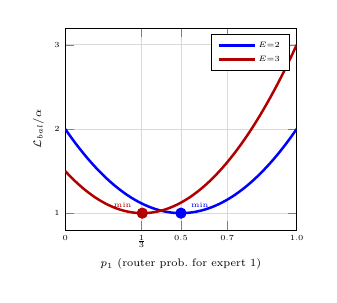
\begin{tikzpicture}[scale=0.75, every node/.style={scale=0.75}]
          \begin{axis}[
            width=5.5cm, height=5cm,
            xlabel={$p_1$ (router prob.\ for expert 1)},
            ylabel={$\mathcal{L}_{\text{bal}} / \alpha$},
            xmin=0, xmax=1, ymin=0.8, ymax=3.2,
            xtick={0, 0.33, 0.5, 0.7, 1.0},
            xticklabels={0, $\frac{1}{3}$, 0.5, 0.7, 1.0},
            grid=major,
            grid style={gray!30},
            every axis label/.style={font=\scriptsize},
            tick label style={font=\tiny},
            legend style={font=\tiny, at={(0.97,0.97)}, anchor=north east},
          ]
            % E=2: L/alpha = E * sum f_i p_i, with f_i = p_i
            % = 2(p^2 + (1-p)^2) = 2(2p^2 - 2p + 1)
            \addplot[blue, very thick, smooth, domain=0:1, samples=50]
              {2*(2*x^2 - 2*x + 1)};
            \addlegendentry{$E{=}2$}

            % E=3: fix p2=p3=(1-p1)/2, f_i=p_i
            % = 3(p1^2 + 2*((1-p1)/2)^2) = 3(p1^2 + (1-p1)^2/2)
            \addplot[red!70!black, very thick, smooth, domain=0:1, samples=50]
              {3*(x^2 + (1-x)^2/2)};
            \addlegendentry{$E{=}3$}

            % Mark minima
            \addplot[mark=*, mark size=2.5pt, blue, only marks] coordinates {(0.5, 1)};
            \addplot[mark=*, mark size=2.5pt, red!70!black, only marks] coordinates {(0.333, 1)};

            % Annotations
            \node[font=\tiny, blue, anchor=south west] at (axis cs:0.52, 1.0) {min};
            \node[font=\tiny, red!70!black, anchor=south east] at (axis cs:0.31, 1.0) {min};
          \end{axis}
        \end{tikzpicture}
      \end{center}

      \vspace{0.1em}
      {\scriptsize Loss as a function of how much probability is concentrated on one expert (others split equally). Minimum at uniform $p_i = 1/E$.}

      \vspace{0.3em}
      \textbf{Trade-off}: Too small $\alpha$ $\Rightarrow$ imbalance; too large $\Rightarrow$ hurts quality by forcing uniformity.
    \end{column}
  \end{columns}
\end{frame}

% -----------------------------------------------------------------------
\begin{frame}{Sparsely-Gated MoE: Hierarchical Gating}

  For very large $E$, a single softmax over all experts dominates the gating cost. \textbf{Hierarchical gating} factorizes routing into two levels.

  \vspace{0.3em}
  \begin{columns}
    \begin{column}{0.4\textwidth}
      \textbf{Flat}: one gate scores all $E$ experts,
      {\small $G(x){=}\mathrm{softmax}(\mathrm{TopK}(xW_g, k))$}, with $W_g\in\mathbb{R}^{d\times E}$.

      \vspace{0.3em}
      \begin{center}
        \begin{tikzpicture}[
          scale=0.6, every node/.style={scale=0.6},
          box/.style={draw, rounded corners, fill=blue!8, minimum width=1.0cm, minimum height=0.5cm, font=\small},
          gate/.style={draw, rounded corners, fill=green!15, minimum width=1.6cm, minimum height=0.5cm, font=\small},
          expert/.style={draw, rounded corners, fill=orange!15, minimum width=0.7cm, minimum height=0.45cm, font=\scriptsize},
          arr/.style={-Stealth, thick},
        ]
          \node[box] (x) at (0,0) {$x$};
          \node[gate] (g) at (0,1.1) {gate $W_g$};
          \draw[arr] (x)--(g);
          \node[expert, fill=gray!15] (e1) at (-2.1,2.6) {$E_1$};
          \node[expert] (e2) at (-1.05,2.6) {$E_2$};
          \node at (0,2.6) {$\cdots$};
          \node[expert, fill=gray!15] (e3) at (1.15,2.6) {$E_{E\text{-}1}$};
          \node[expert] (e4) at (2.3,2.6) {$E_E$};
          \draw[arr,gray!40,thin] (g)--(e1);
          \draw[arr,red!70!black,very thick] (g)--(e2);
          \draw[arr,gray!40,thin] (g)--(e3);
          \draw[arr,red!70!black,very thick] (g)--(e4);
        \end{tikzpicture}
      \end{center}

      {\scriptsize Gating cost $O(E)$ per token.}
    \end{column}
    \begin{column}{0.6\textwidth}
      \textbf{Hierarchical}: a primary gate picks a \emph{group}, a secondary gate picks experts \emph{within} it. Effective weight {\small $G(x)_{(i,j)} = G^{p}(x)_i\,G^{s,i}(x)_j$}.

      \vspace{0.3em}
      \begin{center}
        \begin{tikzpicture}[
          scale=0.6, every node/.style={scale=0.6},
          box/.style={draw, rounded corners, fill=blue!8, minimum width=0.9cm, minimum height=0.5cm, font=\small},
          pg/.style={draw, rounded corners, fill=green!15, minimum width=1.3cm, minimum height=0.6cm, font=\scriptsize, align=center},
          grp/.style={draw, rounded corners, fill=green!8, minimum width=1.1cm, minimum height=0.45cm, font=\scriptsize},
          expert/.style={draw, rounded corners, fill=orange!15, minimum width=0.85cm, minimum height=0.42cm, font=\scriptsize},
          arr/.style={-Stealth, thick},
        ]
          \node[box] (x) at (0,0) {$x$};
          \node[pg] (pg) at (1.7,0) {primary\\ gate};
          \draw[arr] (x)--(pg);
          % groups
          \node[grp] (g1) at (3.6,1.3) {Grp $1$};
          \node[grp, fill=orange!25] (g2) at (3.6,0.1) {Grp $i$};
          \node at (3.6,-0.8) {$\vdots$};
          \node[grp] (gb) at (3.6,-1.6) {Grp $b$};
          \draw[arr,gray!40,thin] (pg)--(g1);
          \draw[arr,red!70!black,very thick] (pg)--(g2);
          \draw[arr,gray!40,thin] (pg)--(gb);
          % experts within selected group
          \node[expert] (a1) at (5.8,0.9) {$E_{i,1}$};
          \node[expert, fill=gray!15] (a2) at (5.8,0.1) {$E_{i,2}$};
          \node at (5.8,-0.6) {$\vdots$};
          \node[expert] (ag) at (5.8,-1.3) {$E_{i,g}$};
          \draw[arr,red!70!black,very thick] (g2)--(a1);
          \draw[arr,gray!40,thin] (g2)--(a2);
          \draw[arr,red!70!black,very thick] (g2)--(ag);
          % labels
          \node[font=\scriptsize, gray] at (3.6,-2.3) {$b$ groups};
          \node[font=\scriptsize, gray] at (5.8,-2.0) {$g$ experts/group};
          \node[font=\scriptsize, align=center] at (5.8,1.8) {secondary gate\\ within Grp $i$};
        \end{tikzpicture}
      \end{center}
    \end{column}
  \end{columns}

  \vspace{0.2em}
  \begin{block}{Cost and capacity}
    $b$ groups $\times$ $g$ experts $= E$ total; top-2 at each level $\Rightarrow 2{\times}2 = 4$ active. Gating cost drops from $O(E)$ to $O(b{+}g)\approx O(\sqrt{E})$. \emph{Example} (100B News): $256 \times 512 = 131{,}072$ experts, yet the router scores only $256{+}512$.
  \end{block}
\end{frame}

% -----------------------------------------------------------------------
\begin{frame}{Sparsely-Gated MoE: Architecture \& Training Details}

  \begin{columns}
    \begin{column}{0.5\textwidth}
      \textbf{Architecture} (language model) \cite{shazeer2017moe}:
      \begin{description}
        \item[Backbone] 5 layers: Embedding $\to$ LSTM $\to$ \textbf{MoE} $\to$ LSTM $\to$ Softmax
        \item[Placement] a \emph{single} MoE layer between the two LSTM layers, applied at every timestep
        \item[Model dim] $d{=}512$ (embedding, LSTM units, MoE input/output)
        \item[Expert] FFN $512\!\to\!1024\!\to\!512$ with ReLU; $\approx$\,1M params each
        \item[Experts/layer] flat 4--256; hierarchical 256--4096 (1B Word); up to \textbf{131{,}072} (100B News, $256{\times}512$ two-level)
        \item[Gating] noisy top-$k$ softmax, $G(x){=}\mathrm{softmax}(\mathrm{TopK}(H(x),k))$
        \item[Active/token] $k{=}4$ flat, or $k{=}2$ per level $\Rightarrow$ 4 experts, $\approx$\,8M ops/timestep
      \end{description}
    \end{column}
    \begin{column}{0.5\textwidth}
      \textbf{Training} (1B Word benchmark):
      \begin{description}
        \item[Optimizer] Adam; lr linear warmup 1k steps, then $\propto 1/\sqrt{\text{step}}$
        \item[Batch] $\approx$\,300k words/batch (large, so each expert sees enough tokens)
        \item[Schedule] 10 epochs ($\approx$\,27k steps)
        \item[Hardware] 16$\times$ K40 GPUs, 12--16\,h/model; experts sharded across GPUs (data $+$ model parallel)
        \item[Dropout] 0.3--0.4 (large models; up to 0.8--0.9 for tiny)
        \item[Load balancing] importance $+$ load auxiliary losses, $w_{\text{imp}}{=}w_{\text{load}}{=}0.1$
        \item[Inference] gating noise disabled $\Rightarrow$ deterministic routing
      \end{description}
    \end{column}
  \end{columns}

  \vspace{0.3em}
  \begin{block}{Key design choice}
    Per-token compute is held near constant ($\approx$\,4 active experts, $\approx$\,8M ops/timestep) while total parameters grow by $>$\,1000$\times$ across the expert sweep.
  \end{block}
\end{frame}

% -----------------------------------------------------------------------
\begin{frame}{Results: Scaling with Sparse MoE}

  \cite{shazeer2017moe} evaluated on language modeling and machine translation:
  {\small (LM metric: test \textbf{perplexity} $=\exp(\text{cross-entropy loss})$; lower is better.)}

  \vspace{0.3em}
  \begin{description}
    \item[Language modeling (1B Word)] MoE \emph{matches or beats} the previous dense state of the art while using only a small fraction of its per-step compute; with more compute it cuts perplexity from \textbf{34.7} (dense SOTA) to \textbf{28.0}.
    \item[Language modeling (100B News)] Perplexity keeps improving with more experts, peaking at \textbf{65{,}536} experts ($\approx$\,$-39\%$ vs.\ baseline), then \emph{reverses} at 131{,}072 once experts become too sparse to each see enough data.
    \item[Machine translation (WMT'14)] New state-of-the-art BLEU on En$\to$Fr and En$\to$De (\textbf{$+1.3$ BLEU} over GNMT) at $\approx$\,$\mathbf{1/6}$ the training time of the production system.
  \end{description}

  \vspace{0.3em}
  \begin{block}{Key takeaway}
    Conditional computation buys $>$\,1000$\times$ model capacity at near-constant per-token compute. The binding constraint at the extreme is not capacity but \emph{per-expert batch size}: too many experts $\Rightarrow$ too little data each $\Rightarrow$ quality regresses.
  \end{block}
\end{frame}

% =======================================================================
\subsection{Switch Transformer}

% -----------------------------------------------------------------------
\begin{frame}{Switch Transformer: Simplifying MoE Routing}

  \cite{fedus2022switch} simplified the MoE approach with two key changes:

  \vspace{0.5em}
  \begin{columns}
    \begin{column}{0.48\textwidth}
      \textbf{1.\ Top-1 routing} (``Switch'' routing):
      \begin{itemize}
        \item Each token goes to \emph{exactly one} expert
        \item Simpler than top-$k$: no need to combine outputs
        \item Reduces communication and computation
      \end{itemize}
      \[
        i^* = \arg\max_i \; (x \cdot W_r)_i
      \]
      \[
        y = G(x)_{i^*} \cdot E_{i^*}(x)
      \]

      \vspace{0.3em}
      \textbf{2.\ Expert capacity factor}:
      \begin{itemize}
        \item Each expert processes at most $C$ tokens per batch
        \item $C = \frac{k \cdot T}{E} \cdot c$, with capacity factor $c > 1$ (e.g.\ $c = 1.25$)
        \item Overflow tokens are passed through residual connection (``dropped'')
      \end{itemize}
    \end{column}
    \begin{column}{0.48\textwidth}
      \begin{center}
        \begin{tikzpicture}[
          scale=0.8, every node/.style={scale=0.8},
          box/.style={draw, rounded corners, fill=blue!8, minimum width=2.8cm, minimum height=0.5cm, align=center, font=\small},
          expert/.style={draw, rounded corners, fill=orange!15, minimum width=1.2cm, minimum height=0.45cm, align=center, font=\small},
          arr/.style={-Stealth, thick},
        ]
          \node[box] (ln) at (0, 0) {LayerNorm};
          \node[box] (attn) at (0, 1.0) {Self-Attention};
          \node[box] (add1) at (0, 2.0) {$+$ (residual)};
          \node[box] (ln2) at (0, 3.0) {LayerNorm};

          % MoE layer
          \draw[thick, dashed, rounded corners, fill=yellow!8] (-2.5, 3.7) rectangle (2.5, 6.3);
          \node[font=\small\bfseries, anchor=north west] at (-2.4, 6.2) {MoE Layer};

          \node[draw, rounded corners, fill=green!15, minimum width=2cm, minimum height=0.4cm, font=\small] (router) at (0, 4.2) {Router};

          \node[expert] (e1) at (-1.5, 5.2) {FFN$_1$};
          \node[expert] (e2) at (0, 5.2) {FFN$_2$};
          \node[expert] (e3) at (1.5, 5.2) {FFN$_3$};

          \node[font=\small] (comb) at (0, 5.9) {weighted output};

          \node[box] (add2) at (0, 6.8) {$+$ (residual)};

          \draw[arr] (ln) -- (attn);
          \draw[arr] (attn) -- (add1);
          \draw[arr] (add1) -- (ln2);
          \draw[arr] (ln2) -- (router);
          \draw[arr, red!70!black] (router) -- (e2);
          \draw[arr, gray!30, thin] (router) -- (e1);
          \draw[arr, gray!30, thin] (router) -- (e3);
          \draw[arr] (comb) -- (add2);
        \end{tikzpicture}
      \end{center}
    \end{column}
  \end{columns}
\end{frame}

% -----------------------------------------------------------------------
\begin{frame}{Switch Transformer: Model Configurations}

  All Switch models are \textbf{FLOP-matched} to their dense T5 counterparts: extra parameters go into expert FFN layers, but only 1 expert is active per token. Quality below is negative log perplexity at 500k steps (higher is better); at matched FLOPs \emph{every} Switch model beats its dense T5 twin.

  \vspace{0.4em}
  \begin{description}
    \item[Switch-Base] 128 experts, \textbf{7.4B} params vs.\ T5-Base's 0.2B at \emph{identical} 124B FLOPs/seq ($37\times$ more params); $-1.306$ vs.\ $-1.556$, and reaches T5-Base quality in \textbf{7$\times$ fewer steps}.
    \item[Switch-Large] 128 experts, \textbf{26B} params vs.\ T5-Large's 0.7B at 425B FLOPs/seq; $-1.177$ vs.\ $-1.350$.
    \item[Switch-XXL] 64 experts, \textbf{395B} params vs.\ T5-XXL's 11B at 6.3T FLOPs/seq; $-1.008$ vs.\ $-1.095$.
    \item[Switch-C] \textbf{1.6T} params, 2048 experts (expert parallelism only $\Rightarrow$ smaller $d_{\text{model}}$, fewer layers); $\sim$\textbf{4$\times$ faster} to T5-XXL quality.
  \end{description}

  \vspace{0.3em}
  \textbf{Training}: 550k steps on C4~\cite{raffel2020t5}, batch size $2^{20}$ tokens, load-balancing coefficient $\alpha_{\text{bal}} = 10^{-2}$.
\end{frame}

% -----------------------------------------------------------------------
\begin{frame}{Switch Transformer: Results}

  \begin{columns}
    \begin{column}{0.50\textwidth}
      \textbf{Pre-training speedup} (FLOP-matched, same hardware):
      \begin{itemize}
        \item Switch-Base reaches T5-Base quality in \textbf{7$\times$ fewer training steps} (60k vs.\ 450k steps, both at 124B FLOPs/seq)
        \item Multilingual: \textbf{5$\times$ mean step speedup} over mT5-Base across 101 languages
        \item Switch-C reaches T5-XXL quality in $\sim$\textbf{4$\times$ fewer steps} in wall-clock time, but \emph{not} FLOP-matched (890B vs.\ 6.3T FLOPs/seq)
      \end{itemize}

      \vspace{0.3em}
      \textbf{Downstream tasks} (fine-tuning):
      \begin{itemize}
        \item SuperGLUE: 75.1 (T5-Base) $\to$ \textbf{79.5} (Switch-Base)
        \item Winogrande: 66.6 $\to$ \textbf{73.3}
        \item XSum: 18.7 $\to$ \textbf{20.3}
      \end{itemize}
    \end{column}
    \begin{column}{0.46\textwidth}
      \textbf{Training stability mitigations}:
      \begin{itemize}
        \item \textbf{Selective precision}: router computation in \texttt{float32}, rest in \texttt{bfloat16}. Pure \texttt{bfloat16} diverges; selective precision matches \texttt{float32} quality at \texttt{bfloat16} speed
        \item \textbf{Reduced init scale}: weights $W\sim\mathcal{N}(0,\,s/n)$ ($n=$ fan-in); $s = 0.1$ (10$\times$ smaller than default). With $s=1.0$: high variance, unstable
        \item \textbf{Expert dropout}: 0.4 at expert layers during fine-tuning (vs.\ 0.1 elsewhere)
      \end{itemize}

      \vspace{0.3em}
      \begin{block}{Design Principles}
        \begin{enumerate}
          \item Top-1 routing is sufficient
          \item More experts $>$ larger experts
          \item Auxiliary loss for load balancing
          \item Numerical precision matters
        \end{enumerate}
      \end{block}
    \end{column}
  \end{columns}
\end{frame}

% =======================================================================
\subsection{DeepSeek-MoE}

% -----------------------------------------------------------------------
\begin{frame}{DeepSeek-MoE: Fine-Grained Expert Specialization}

  \cite{dai2024deepseekmoe} proposed two innovations to improve expert specialization:

  \vspace{0.5em}
  \begin{columns}
    \begin{column}{0.48\textwidth}
      \textbf{1.\ Fine-grained expert segmentation}:
      \begin{itemize}
        \item Instead of $E$ large experts, split into $mE$ smaller experts (each $1/m$ the size)
        \item Activate $mk$ experts (same total compute)
        \item Allows more flexible, fine-grained combinations of knowledge
      \end{itemize}

      \vspace{0.3em}
      \textbf{Example}: Instead of 16 experts with top-2, use 64 experts with top-8 (same compute, more combinatorial flexibility).

    \end{column}
    \begin{column}{0.48\textwidth}
      \textbf{2.\ Shared experts}:
      \begin{itemize}
        \item Dedicate $K_s$ experts as \textbf{shared}, always active for every token
        \item Remaining experts are \textbf{routed} as usual
        \item Shared experts capture common knowledge; routed experts specialize
      \end{itemize}

      \vspace{0.3em}
      \begin{block}{Output}
        \vspace{-0.3em}
        \[
          y = \sum_{i=1}^{K_s} E^{(s)}_i(x) + \sum_{i \in \text{top-}k} g_i \cdot E^{(r)}_i(x)
        \]
      \end{block}
    \end{column}
  \end{columns}
\end{frame}

% -----------------------------------------------------------------------
\begin{frame}{DeepSeek-MoE: Architecture}

  \begin{center}
    \begin{tikzpicture}[
      scale=0.85, every node/.style={scale=0.85},
      shared/.style={draw, rounded corners, fill=green!20, minimum width=1.0cm, minimum height=0.45cm, align=center, font=\scriptsize},
      routed/.style={draw, rounded corners, fill=orange!20, minimum width=0.7cm, minimum height=0.45cm, align=center, font=\scriptsize},
      gate/.style={draw, rounded corners, fill=blue!15, minimum width=1.8cm, minimum height=0.45cm, align=center, font=\small},
      arr/.style={-Stealth, thick},
    ]
      % Input
      \node[font=\small] (input) at (0, 0) {Token $x$};

      % Shared experts (always active)
      \node[shared] (s1) at (-4.5, 2.5) {Shared 1};
      \node[shared] (s2) at (-3.0, 2.5) {Shared 2};

      % Router
      \node[gate] (router) at (1.5, 1.2) {Router};

      % Routed experts
      \node[routed] (r1) at (-0.8, 2.5) {$E_1$};
      \node[routed] (r2) at (0.4, 2.5) {$E_2$};
      \node[routed] (r3) at (1.6, 2.5) {$E_3$};
      \node[font=\small] at (2.6, 2.5) {$\cdots$};
      \node[routed] (rn) at (3.7, 2.5) {$E_{mE}$};

      % Connections
      \draw[arr, green!50!black, very thick] (input) -- (s1);
      \draw[arr, green!50!black, very thick] (input) -- (s2);
      \draw[arr] (input) -- (router);
      \draw[arr, red!70!black, very thick] (router) -- (r1);
      \draw[arr, gray!30, thin] (router) -- (r2);
      \draw[arr, red!70!black, very thick] (router) -- (r3);
      \draw[arr, gray!30, thin] (router) -- (rn);

      % Sum node
      \node[draw, circle, fill=yellow!15, inner sep=2pt, font=\small] (sum) at (0, 3.8) {$\Sigma$};
      \draw[arr, green!50!black, very thick] (s1) -- (sum);
      \draw[arr, green!50!black, very thick] (s2) -- (sum);
      \draw[arr, red!70!black, very thick] (r1) -- (sum);
      \draw[arr, red!70!black, very thick] (r3) -- (sum);

      % Output
      \node[font=\small] (output) at (0, 4.6) {Output $y$};
      \draw[arr] (sum) -- (output);

      % Labels
      \draw[thick, green!50!black, dashed] (-5.2, 1.8) rectangle (-2.3, 3.1);
      \node[font=\scriptsize, green!50!black, anchor=north] at (-3.75, 1.75) {always active};

      \draw[thick, orange!70!black, dashed] (-1.3, 1.8) rectangle (4.3, 3.1);
      \node[font=\scriptsize, orange!70!black, anchor=north] at (1.5, 1.75) {top-$k$ routed};
    \end{tikzpicture}
  \end{center}

  \vspace{0.2em}
  \begin{itemize}
    \item Shared experts reduce \emph{redundancy} among routed experts
    \item Fine-grained segmentation provides $\binom{mE}{mk}$ possible expert combinations vs.\ $\binom{E}{k}$ with standard MoE
  \end{itemize}
\end{frame}

% -----------------------------------------------------------------------
\begin{frame}{DeepSeek-MoE: Architecture \& Training Details}

  \begin{columns}
    \begin{column}{0.5\textwidth}
      \textbf{Architecture} (16B; 145B in parens) \cite{dai2024deepseekmoe}:
      \begin{description}
        \item[Backbone] decoder-only Transformer, \textbf{28} (62) layers, $d_{\text{model}}{=}2048$ (4096), 16 (32) heads of dim 128; RoPE, RMSNorm, SwiGLU
        \item[MoE placement] every FFN is an MoE layer \emph{except the first} (kept dense -- its load balance converges slowest)
        \item[Experts/layer] \textbf{2 shared $+$ 64 routed} (4 $+$ 128), each $1/m$ of a standard FFN, $m{=}4$ ($m{=}8$)
        \item[Routing] all shared $+$ top-\textbf{6} of 64 (top-12 of 128) $\Rightarrow$ 8 (16) active experts/token
        \item[Size] 16.4B total / \textbf{2.8B active} (144.6B / 22.2B)
      \end{description}
    \end{column}
    \begin{column}{0.5\textwidth}
      \textbf{Training} (16B):
      \begin{description}
        \item[Data] \textbf{2T} tokens, sequence length 4096
        \item[Optimizer] AdamW ($\beta_1{=}0.9,\beta_2{=}0.95$, wd $0.1$), grad-clip 1.0
        \item[LR] max $4.2\times10^{-4}$; linear warmup 2k steps, then $\times0.316$ at 80\% and 90\% of steps (multi-step decay)
        \item[Batch] 4.5k sequences $\approx$ \textbf{18M} tokens/batch
        \item[Load balancing] expert-level balance loss ($\alpha{=}10^{-3}$); no device-level loss for 16B (145B adds device-level $0.05$)
      \end{description}
    \end{column}
  \end{columns}

  \vspace{0.3em}
  \begin{block}{Key choice}
    Always-on shared experts plus fine-grained routed experts ($m{=}4$) let \textbf{2.8B} active params match a $\sim$7B dense model.
  \end{block}
\end{frame}

% -----------------------------------------------------------------------
\begin{frame}{DeepSeek-MoE: Results}

  \begin{columns}
    \begin{column}{0.50\textwidth}
      \textbf{DeepSeek-MoE 16B} (2.8B active):
      \begin{itemize}
        \item Comparable to LLaMA-2 7B and DeepSeek 7B dense
        \item $\approx$\textbf{40\%} of the compute of an equivalent dense model
        \item Active params: 2.8B vs.\ 6.9B dense
      \end{itemize}

      \vspace{0.3em}
      \textbf{DeepSeek-MoE 145B} (22.2B active):
      \begin{itemize}
        \item Approaches DeepSeek 67B dense performance
        \item Only \textbf{1/3} the active params (22.2B vs.\ 67B)
        \item Confirms fine-grained + shared experts scale
      \end{itemize}
    \end{column}
    \begin{column}{0.46\textwidth}
      \textbf{Ablation results} ($m = 4$ best):
      \begin{itemize}
        \item Fine-grained segmentation alone: significant gain over standard top-$k$ MoE
        \item Shared experts alone: moderate gain
        \item Combined: largest improvement
        \item $\binom{64}{6} \approx 74$M combinations vs.\ $\binom{16}{2} = 120$ for standard MoE
      \end{itemize}

      \vspace{0.3em}
      \begin{block}{Design Recipe}
        Fine-grained segmentation ($m{=}4$) + shared experts ($K_s{=}2$) consistently outperforms standard MoE and dense models at matched compute.
      \end{block}
    \end{column}
  \end{columns}
\end{frame}

% =======================================================================
\subsection{DeepSeek-V3: MoE at Scale}

% -----------------------------------------------------------------------
\begin{frame}{DeepSeek-V3: Auxiliary-Loss-Free Load Balancing}

  \cite{deepseekai2024deepseekv3} identified a key problem with auxiliary balancing losses:

  \vspace{0.3em}
  \begin{alertblock}{Problem}
    The auxiliary loss $\mathcal{L}_{\text{bal}}$ conflicts with the language modeling objective. Tuning $\alpha$ is difficult: too small $\Rightarrow$ imbalance, too large $\Rightarrow$ hurts model quality.
  \end{alertblock}

  \vspace{0.3em}
  \textbf{Solution: Bias-based load balancing} (no auxiliary loss):

  \begin{itemize}
    \item Add a learnable \textbf{bias} term $b_i$ to each expert's gating score for routing:
    \[
      i^* = \arg\max_i \; \big(s_i(x) + b_i\big)
    \]
    \item The bias is \textbf{not} used in the gating weight (only for routing decisions):
    \[
      g_i(x) = \frac{s_i(x)}{\sum_{j \in \text{top-}k} s_j(x)}
    \]
    \item $b_i$ is adjusted dynamically: if expert $i$ is overloaded, decrease $b_i$; if underloaded, increase $b_i$
  \end{itemize}

  $\Rightarrow$ Load balancing is \emph{decoupled} from the training loss.
\end{frame}

% -----------------------------------------------------------------------
\begin{frame}{DeepSeek-V3: Architecture Overview}

  \textbf{DeepSeek-V3}: 671B total parameters, 37B active per token.

  \vspace{0.5em}
  \begin{columns}
    \begin{column}{0.48\textwidth}
      \textbf{MoE configuration}:
      \begin{itemize}
        \item 61 Transformer layers
        \item First 3 layers: dense FFN
        \item Layers 4--61: MoE layers
        \item 256 routed experts + 1 shared expert per MoE layer
        \item Top-8 routing (out of 256)
        \item Fine-grained segmentation following DeepSeek-MoE
      \end{itemize}

      \vspace{0.3em}
      \textbf{Additional innovations}:
      \begin{itemize}
        \item Multi-head Latent Attention (MLA) for KV cache compression
        \item Multi-token prediction as auxiliary training objective
        \item FP8 mixed-precision training
      \end{itemize}
    \end{column}
    \begin{column}{0.48\textwidth}
      \textbf{Training efficiency}:
      \begin{itemize}
        \item Trained on 14.8T tokens
        \item Training cost: \textbf{2.788M H800 GPU hours}
        \item $\approx$\$5.5M (remarkably economical)
        \item Comparable to GPT-4 / LLaMA-3 405B quality
      \end{itemize}

      \vspace{0.3em}
      \begin{block}{Why so efficient?}
        \begin{itemize}
          \item MoE: only 37B of 671B params active
          \item FP8 training: $\sim$2$\times$ throughput vs.\ BF16
          \item Efficient expert parallelism with minimal communication
        \end{itemize}
      \end{block}
    \end{column}
  \end{columns}
\end{frame}

% =======================================================================
\subsection{Summary}

% -----------------------------------------------------------------------
\begin{frame}{MoE: Summary and Open Challenges}

  \textbf{Key ideas}:
  \begin{itemize}
    \item MoE \emph{decouples} model capacity (total params) from compute cost (active params)
    \item Router selects a sparse subset of experts per token
    \item Load balancing is essential for training stability and efficiency
  \end{itemize}

  \vspace{0.5em}
  \textbf{Evolution}:
  \begin{itemize}
    \item \textbf{Shazeer (2017)}: Sparsely-gated MoE layer, noisy top-$k$ gating, auxiliary loss
    \item \textbf{Switch (2022)}: Simplified top-1 routing, scaled to 1.6T params
    \item \textbf{DeepSeek-MoE (2024)}: Fine-grained experts + shared experts
    \item \textbf{DeepSeek-V3 (2024)}: Auxiliary-loss-free balancing, 671B params at low cost
  \end{itemize}

  \vspace{0.3em}
  \textbf{Open challenges}:
  \begin{itemize}
    \item \textbf{Inference}: All expert weights must be in memory, even though most are idle
    \item \textbf{Expert collapse}: Some experts may remain underutilized
    \item \textbf{Communication}: Expert parallelism requires all-to-all communication
    \item \textbf{Distillation}: Can we compress MoE back into smaller dense models?
  \end{itemize}
\end{frame}
